\documentclass[conference]{IEEEtran}
\usepackage{times}

% numbers option provides compact numerical references in the text.
\usepackage[numbers]{natbib}
\usepackage{multicol}
\usepackage[bookmarks=true]{hyperref}
\usepackage{amsmath,amssymb}
% \usepackage[standard]{ntheorem}
\usepackage{amsthm}
\usepackage{mathtools}
\usepackage{graphicx}
% \usepackage{caption}
% \usepackage{figure}
\usepackage{float}
\usepackage{subcaption}
\usepackage{epstopdf}
\usepackage{dblfloatfix}
\usepackage{fixltx2e}
% \usepackage{subfig}
\usepackage{algorithm}
\usepackage{algorithmicx}
\usepackage[noend]{algpseudocode}
\makeatletter
\def\BState{\State\hskip-\ALG@thistlm}
\makeatother
\algdef{SE}[DOWHILE]{Do}{DoWhile}[1]{\algorithmicdo\ #1}[1]{\algorithmicwhile\ #1}

\usepackage{tabstackengine}
\stackMath

\usepackage{tikz}
\usetikzlibrary{scopes}
\usetikzlibrary{shapes.misc}
\tikzset{cross/.style={cross out, draw=black, minimum size=2*(#1-\pgflinewidth), inner sep=0pt, outer sep=0pt},
%default radius will be 1pt.
cross/.default={2pt}}


\newtheorem{theorem}{Theorem}
\newtheorem{proposition}{Proposition}
\newtheorem{corollary}{Corollary}
\newcommand\numberthis{\addtocounter{equation}{1}\tag{\theequation}}
\DeclareMathOperator{\sign}{\text{sgn}}
\DeclareMathOperator*{\argmin}{arg\,min}
\DeclareMathOperator{\intr}{int}
\DeclareMathOperator{\dom}{dom}

\newcommand{\EH}[1]{{\color{blue} {Eric: {#1}}  }}
\newcommand{\TODO}[1]{{\color{red} {{#1}}  }}

\pdfinfo{
   /Author (Eric Huang)
   /Title  (Robots: Our new overlords)
   /CreationDate (D:20161016120000)
   /Subject (Robots)
   /Keywords (Robots;Overlords)
}

\begin{document}

% paper title
\title{Robotic Pulling}

% You will get a Paper-ID when submitting a pdf file to the conference system
% \author{Author Names Omitted for Anonymous Review. Paper-ID [add your ID here]}

%\author{\authorblockN{Michael Shell}
%\authorblockA{School of Electrical and\\Computer Engineering\\
%Georgia Institute of Technology\\
%Atlanta, Georgia 30332--0250\\
%Email: mshell@ece.gatech.edu}
%\and
%\authorblockN{Homer Simpson}
%\authorblockA{Twentieth Century Fox\\
%Springfield, USA\\
%Email: homer@thesimpsons.com}
%\and
%\authorblockN{James Kirk\\ and Montgomery Scott}
%\authorblockA{Starfleet Academy\\
%San Francisco, California 96678-2391\\
%Telephone: (800) 555--1212\\
%Fax: (888) 555--1212}}


% avoiding spaces at the end of the author lines is not a problem with
% conference papers because we don't use \thanks or \IEEEmembership


% for over three affiliations, or if they all won't fit within the width
% of the page, use this alternative format:
% 
%\author{\authorblockN{Michael Shell\authorrefmark{1},
%Homer Simpson\authorrefmark{2},
%James Kirk\authorrefmark{3}, 
%Montgomery Scott\authorrefmark{3} and
%Eldon Tyrell\authorrefmark{4}}
%\authorblockA{\authorrefmark{1}School of Electrical and Computer Engineering\\
%Georgia Institute of Technology,
%Atlanta, Georgia 30332--0250\\ Email: mshell@ece.gatech.edu}
%\authorblockA{\authorrefmark{2}Twentieth Century Fox, Springfield, USA\\
%Email: homer@thesimpsons.com}
%\authorblockA{\authorrefmark{3}Starfleet Academy, San Francisco, California 96678-2391\\
%Telephone: (800) 555--1212, Fax: (888) 555--1212}
%\authorblockA{\authorrefmark{4}Tyrell Inc., 123 Replicant Street, Los Angeles, California 90210--4321}}


\maketitle

\begin{abstract}

% Items that an abstract should address:
% 1. What were the main contributions?
% 2. 
% 3. 

Planar pulling is the manipulation skill where
the robot contacts a rigid body at a point and pulls that contact
point along a trajectory.

Major contributions:
  \begin{enumerate}
  \item Proof of stability
  \item first known algorithm that computes exact angular velocity
    bounds on the friction dominated motion of a pushed/pulled object.
  \item Uncertainty bounds on the orientation
  \item Planner that exploits the stability of pulling using the exact
    angular velocity bounds.
  \item to return trajectories.
  \item An easy to implement in both hardware and software skill. 
  \item validated on a real robotic system.

    A useful addition to a roboticist's toolkit. that is serviceable
    in a wide range of scenarios. ranging from furniture rearrangement
    or table-top manipulation to bin picking.
  \end{enumerate}
\end{abstract}

\IEEEpeerreviewmaketitle

\section{Introduction}

% Items that an introduction should address:
% 1. 
% 2. 

In this paper, we demonstrate the value of 

\begin{enumerate}
\item Looking at pushing from a different perspective
\item contributions
\item open-loop stable with convergence guarantees
\item easy to use
\item Outline of sections
\end{enumerate}

\section{Related Work}

\TODO{
Items that a related works section should address:
\begin{enumerate}
\item What were the prior works?
\item What were the limitations of the prior works?
\item What are the advantages of our work?
\end{enumerate}
}


\begin{enumerate}
\item Planar Robotic Manipulation
  \begin{enumerate}
  \item Pushing
  \item Tapping
  \item Throwing
  \item Grasping
  \item Pivoting
  \item Why pulling over other planar manipulation skills
  \end{enumerate}
\item Robotic Pushing
  \begin{enumerate}
  \item Planning
  \item Force-motion model
  \item Quasi-static motion model
  \item Stable pushing
  \end{enumerate}

  Our work is most closely related to robotic pushing.

  Lynch 

  two-point stable pushing of Lynch et al. \cite{}.

  mechanical components robust to variations in the friction

\item Pushing Bounds

  \begin{enumerate}
  \item Bisector bound
  \item Vertical strip bound
  \item Alexander and Maddocks bound
  \item Peshkin's bound
  \end{enumerate}

\item Holonomic Planning
\item DDP
\item Uncertainty reduction
\item Stability
\end{enumerate}







The problem of finding exact angular velocity bounds for a pushed
object with an indeterminant pressure distribution was first raised in
Mason's seminal thesis on robotic pushing \cite{Mason1982}. Since
then, various inexact angular velocity bounds have been published.
The bisector bound restricts the feasible rotation centers to a
half-space delimited by the perpendicular bisector between the contact
point and center of pressure \cite{Mason}.  Alexander and Maddock
bounded the set of feasible rotation centers to lie within the minimum
object-enclosing vertical strip perpendicular to the wrench applied by
the pusher \cite{alexander1993bounds}.  Peshkin bounded the motion of
a pushed object by computing the set of feasible rotation centers of
the minimum object-enclosing disk centered at the object's center of
pressure \cite{peshkin1988motion}.  In contrast to the prior art, our
algorithm is the first to find \textit{exact} angular velocity bounds
for a pushed object.



\section{Theory}

\subsection{Planar Pulling Subject to Friction}\label{sec:planar-pulling}

We present a preliminary quasi-static analysis of planar pulling
subject to friction. Planar pulling is the manipulation skill where
the robot contacts a rigid body at a point and pulls that contact
point along a trajectory.

Let the \textit{generalized velocity} of a planar rigid body be
$\mathbf{v}^+ = [v_x, v_y, \omega]^T$, where $v_x$ and $v_y$ are the
linear velocities of a reference point and $\omega$ is the angular
velocity about that point. Taking the origin as the reference point,
the velocity of a point $\mathbf{x}$ on the body is then given by
$\mathbf{v}(\mathbf{x}) = [v_x, v_y]^T + \omega\hat{\mathbf{k}} \times
\mathbf{x}$ and can be written in matrix notation as
\begin{equation} \label{eq:generalized-velocity}
\mathbf{v}(\mathbf{x}) = A(\mathbf{x})\mathbf{v}^+,
\end{equation}
where
\begin{equation}
  A(\mathbf{x}) = 
  \begin{bmatrix*}[r]
    1 & 0 & -x_2 \\
    0 & 1 &  x_1
  \end{bmatrix*}.
\end{equation}

In this analysis, we choose a coordinate frame such that the origin is
the contact point and the $y$-axis aligns with the contact point
velocity (see Figure \ref{fig:presspull-motion} for an example). Then
the total frictional force and moment of the body at the origin are
\begin{align}
  % Force
  % \mathbf{f}_f &= -\mu\,\sign(\dot{\theta})\,\mathbf{\hat{k}}\,\times\int_{R}\frac{\mathbf{r}-\mathbf{r_{\text{IC}}}}{\lVert \mathbf{r}-\mathbf{r_{\text{IC}}} \rVert} p(\mathbf{r}) dA \\
  \mathbf{f}_f &= -\mu\int_{R}\frac{A(\mathbf{r})\mathbf{v}^+}{\lVert A(\mathbf{r})\mathbf{v}^+ \rVert} p(\mathbf{r}) dA \\
  % \mathbf{f}_f &= -\mu\int_{R}\frac{\mathbf{v}(\mathbf{r})}{\lVert \mathbf{v}(\mathbf{r}) \rVert} p(\mathbf{r}) dA \\
  % Moment
  % \mathbf{m}_f &= -\mu\,\sign(\dot{\theta}) \int_{R}\mathbf{r}\cdot\frac{\mathbf{r}-\mathbf{r_{\text{IC}}}}{\lVert \mathbf{r}-\mathbf{r_{\text{IC}}} \rVert} p(\mathbf{r}) dA,
  \mathbf{m}_f &= -\mu\int_{R}\mathbf{r}\times\frac{A(\mathbf{r})\mathbf{v}^+}{\lVert A(\mathbf{r})\mathbf{v}^+ \rVert} p(\mathbf{r}) dA, \label{eq:moment-at-contact}
  % \mathbf{m}_f &= -\mu\int_{R}\mathbf{r}\times\frac{\mathbf{v}(\mathbf{r})}{\lVert \mathbf{v}(\mathbf{r}) \rVert} p(\mathbf{r}) dA, \label{eq:moment-at-contact}
\end{align}
where $\mu$ is the coefficient of friction, $R$ is the region of the
rigid body in contact with the plane, $\mathbf{v}(\mathbf{r})$ is the
body point velocity given by (\ref{eq:generalized-velocity}) and
$p(\mathbf{r})$ is a pressure distribution over $R$.

The principle of minimal dissipation states that the motion of the
pulled body minimizes the instantaneous work dissipated by friction
\cite{alexander1993bounds}. That is, the motion minimizes the
following: 
\begin{equation}
\begin{aligned}
& \underset{\mathbf{v}^+}{\text{minimize}}
& & \mu\int_R\lVert A(\mathbf{r})\mathbf{v}^+ \rVert p(\mathbf{r}) dA \\
& \text{subject to}
& & \mathbf{v}^+ \in \mathcal{C}.
\end{aligned} \label{eq:constrained-frictional-dissipation}
\end{equation}
Without loss of generality, we take
$\mathcal{C} = \{[0,1,\omega]^T, \omega \in \mathbb{R}\}$ so that the
contact point motion is aligned with the coordinate frame. We call the
objective in (\ref{eq:constrained-frictional-dissipation}) the
frictional dissipation equation $\mathrm{P}(\mathbf{v}^+)$.

The principle of minimal dissipation is equivalent to the quasi-static
model of planar sliding with friction \cite{alexander1993bounds}.  In
fact, the quasi-static model is identical to the first order
optimality conditions of
(\ref{eq:constrained-frictional-dissipation}). To see this, take the
Lagrangian of (\ref{eq:constrained-frictional-dissipation})
\begin{equation}
  \mathrm{L}(\mathbf{v}^+,\mathbf{\lambda}) = \mathrm{P}(\mathbf{v}^+) + \lambda_1v^+_1 + \lambda_2(v^+_2-1)
\end{equation}
and set gradient of $\mathrm{L}$ with respect to $\mathbf{v}^+$,
\begin{equation}
  \nabla\mathrm{L}(\mathbf{v}^+,\mathbf{\lambda}) = \mu\int_R\frac{A(\mathbf{r})^TA(\mathbf{r})\mathbf{v}^+}{\lVert A(\mathbf{r})\mathbf{v}^+ \rVert} p(\mathbf{r}) dA + \begin{bmatrix}\lambda_1, \lambda_2, 0\end{bmatrix}^T,
\end{equation}
to zero. After some work, we end up with the following first order
conditions on the force and the moment
\begin{align}
  \mathbf{f}_f &= \begin{bmatrix}\lambda_1, \lambda_2\end{bmatrix}^T\\
  \mathbf{m}_f &= 0,
\end{align}
that is, the quasi-static motion model.

We prefer the principle of minimal dissipation in our theoretical
analysis because the frictional dissipation equation is continuous and
convex in $\mu$, $p(\mathbf{x})$ and $\mathbf{v}^+$.

\subsection{Quasi-static Stability}

% Press-pull stability theorem figure.
\begin{figure}
  \centering
  \def\iangle{35} % Angle of the inclined plane
  \begin{tikzpicture}[
    scale=1.25, every node/.style={scale=1.25},
    force/.style={>=latex,draw=black,fill=black},
    axis/.style={densely dashed,draw=gray,font=\small},
    ]
    \fill[draw=black,fill=blue!10,thin,rotate=\iangle] (-0.3,-0.5) rectangle (2.3,.5);
    \draw[rotate=\iangle] (1,0) circle[radius=2.4pt] node[cross] {};
    \draw[rotate=\iangle] (1,0) node[above right] {\tiny CoP};
    {[axis,->]
      \draw (0,0) -- (2.5,0) node[right] {$x$};
      \draw (0,0) -- (0,2.5) node[above] {$y$};
    }
    {[force,->]
      \draw (0,0) -- ++(0,1.5) node[right] {$\mathbf{v}_c$};
    }
    \fill (0,0) circle [radius=1.pt];
    \fill (1.2207,0) circle [radius=1.pt] node[below right] {$x_{\text{\tiny IC}}$};
  \end{tikzpicture}
  \caption{Motion of a press-pulled slider.}
  \label{fig:presspull-motion}
\end{figure}

\begin{theorem}
  For pulling of a rigid body in the plane, the line from the pulling
  contact point to the body's center of pressure converges to the line
  of motion.
\end{theorem}

\begin{proof}
  % TODO Shorten this proof. Rewrite to use generalized velocities.
  Let the $y$-axis of the coordinate frame be aligned with the line of
  motion of the press-pull contact point (see Figure
  \ref{fig:presspull-motion} for an example). Then the instantaneous
  rotation center of the body must fall on the $x$-axis, and we can
  write $\mathbf{r}_\text{IC} = (x_\text{IC},0)^T$.

  Suppose the center of pressure is strictly to the right of the line
  of motion (as in Figure \ref{fig:presspull-motion}). Then by Theorem
  7.4 in \cite{Mason}, the rotation center lies on the positive
  $x$-axis and has negative rotation. The velocity of a point on the
  rigid body is given by
  $\mathbf{v}(\mathbf{r}) =
  \dot{\theta}\,\hat{\mathbf{k}}\times(\mathbf{r} -
  \mathbf{r}_\text{IC})$.
  We can compute the motion of the body relative to the contact point
  by
  \begin{align*}
    \mathbf{v}(\mathbf{r}) - \mathbf{v}_c &= \dot{\theta}\,\hat{\mathbf{k}}\times(\mathbf{r} - \mathbf{r}_\text{IC}) - \dot{\theta}\,\hat{\mathbf{k}}\times(\mathbf{0} - \mathbf{r}_\text{IC}) \\
    &= \dot{\theta}\,\hat{\mathbf{k}}\times(\mathbf{r} - \mathbf{0}) \numberthis \label{eqn:rel-rotation-center},
  \end{align*}
  where $\mathbf{v}_c$ is the velocity of the contact point. In other
  words, the body is rotating clockwise relative to the
  contact point with angular velocity
  \begin{equation}
    \dot{\theta} = -\frac{\lVert\mathbf{v}_c\rVert}{x_\text{IC}}.
  \end{equation}

  Let $\theta \in (\pi/2, -\pi/2)$ be the orientation of the center of
  pressure in the frame of the contact point. When the line of motion
  passes through the center of pressure, a pure translation takes
  place (Theorem 7.4 in \cite{Mason}). This implies that
  $\dot{\theta} = 0$ if and only if $\theta = \pi/2, -\pi/2$. Since
  $\theta$ is monotonically decreasing, we see that it must converge
  to $-\pi/2$ in the limit as $t \rightarrow \infty$.

  The case when the center of pressure is strictly to the left of the
  line of motion follows from symmetry about the $y$-axis.
\end{proof}

Note that the above proof holds for \textit{all pressure
  distributions} of the body on the support
surface.

% \begin{proposition}
%   When pressing down on a point contact on a rigid body, the center of
%   pressure is given by
%   \begin{equation}
%     \text{CoP} = \frac{1}{f_0 + p_c}\left(\int_R\mathbf{r}p(\mathbf{r})dA + \mathbf{r}_cp_c\right)
%   \end{equation}
% \end{proposition}
% In other words, the resulting center of pressure is located on the
% line segment between the contact point and the original center of
% pressure. 

% \begin{proposition}
%   A rigid body in the plane can be moved from A to B with arbitrary
%   accuracy using at most two press-pulls.
% \end{proposition}

\subsection{Frictional Force \& Moment Envelopes}\label{sec:frictional-envelope}

\begin{figure}[t]
  \centering
  \begin{subfigure}[b]{0.24\textwidth}
    \centering
    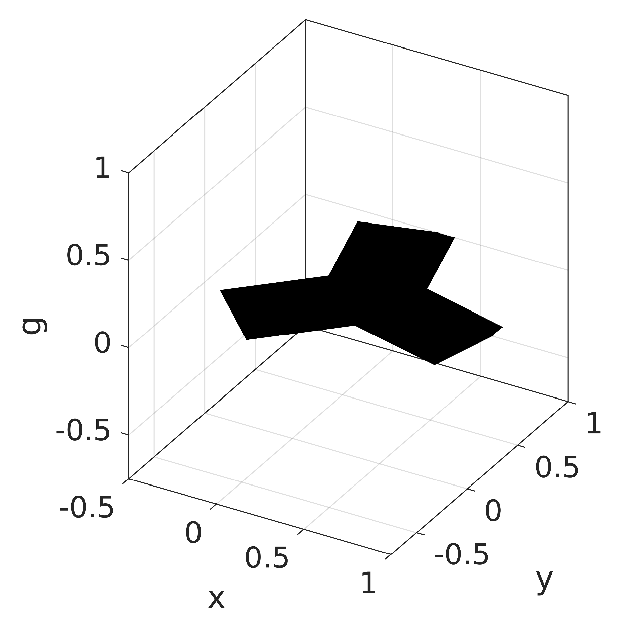
\includegraphics[width=1\linewidth]{./fig/moment_hull_1}
    \caption{}
  \end{subfigure}
  \begin{subfigure}[b]{0.24\textwidth}
    \centering
    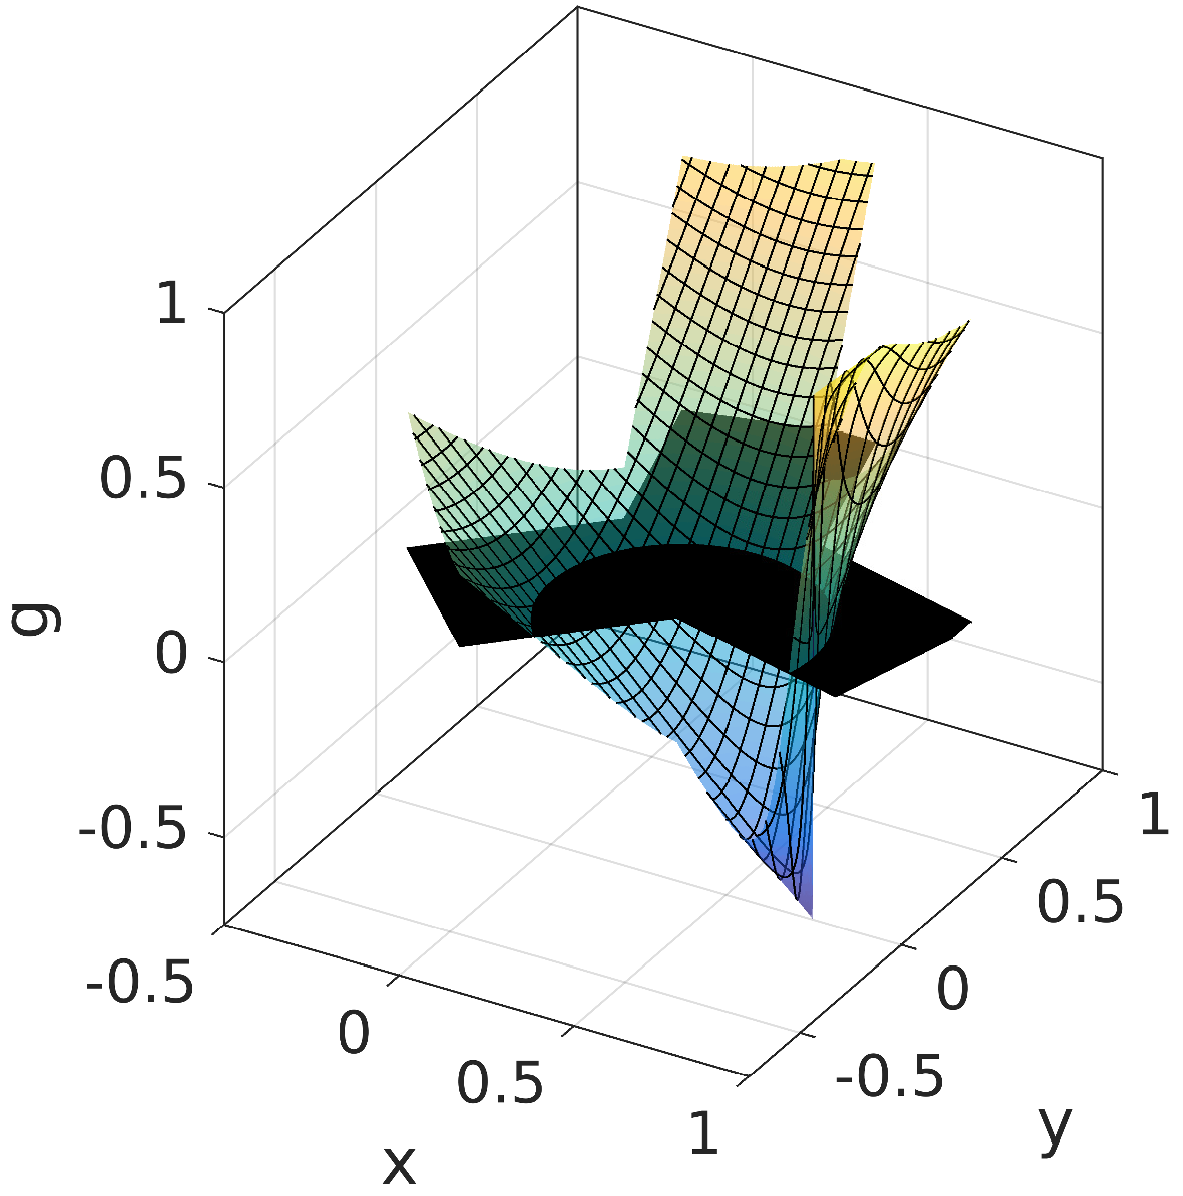
\includegraphics[width=1\linewidth]{fig/moment_hull_2}
    \caption{}
  \end{subfigure}
  \begin{subfigure}[b]{0.24\textwidth}
    \centering
    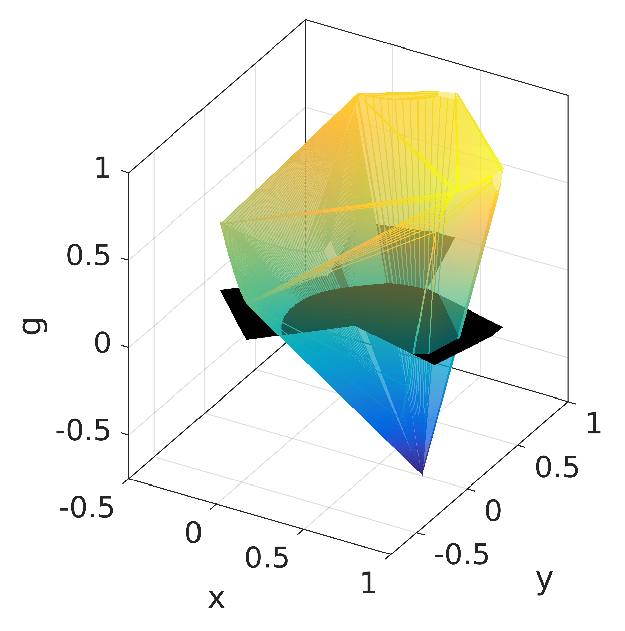
\includegraphics[width=1\linewidth]{fig/moment_hull_3}
    \caption{}
  \end{subfigure}
  \begin{subfigure}[b]{0.24\textwidth}
    \centering
    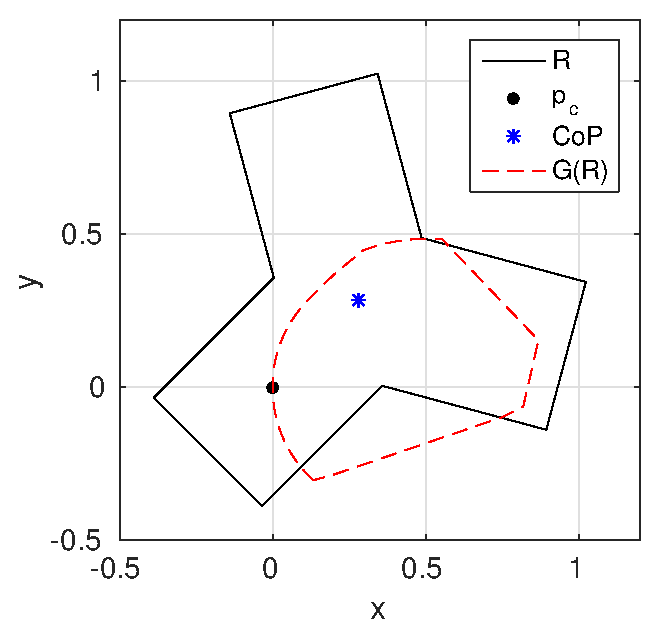
\includegraphics[width=1\linewidth]{fig/CoP_boundary}
    \caption{}
  \end{subfigure}
  \caption{Example moment envelope for a 2D tetrapod with rotation
    center $x_{\text{IC}} = 0.75$. (a) Support region $R$. (b)
    Normalized-moment surface $G(R)$. (c) Convex moment envelope of
    $G(R)$. (d) Intersection of the moment envelope and the
    $xy$-plane. The intersection bounds the set of feasible centers of
    pressure with zero moment.}
  \label{fig:moment-envelope}
\end{figure}

The frictional force and moment envelopes provide a nice geometric
model of the constraints between the center of pressure, force and
moment \cite{Mason}. A frictional envelope has as its parameters the
support region $R$ and the velocity $\mathbf{v}^+$.  Let $f_0$ be the
total pressure. Then the functions
\begin{align}
  \mathbf{f}(\mathbf{x}) &= -\mu f_0\,\frac{A(\mathbf{x})\mathbf{v}^+}{\lVert A(\mathbf{x})\mathbf{v}^+ \rVert},\\
  g(\mathbf{x}) &= -\mu f_0\,\mathbf{x}\times \frac{A(\mathbf{x})\mathbf{v}^+}{\lVert A(\mathbf{x})\mathbf{v}^+ \rVert} \label{eq:unit-moment-at-x}
\end{align}
evaluate the frictional force and frictional torque that would result
from a unit normalized pressure at $\mathbf{x}$. For this exposition,
we will focus on how to generate the frictional moment envelope
illustrated in Figure \ref{fig:moment-envelope}.

Let $G$ map $R$ into a surface in $\mathbb{R}^3$ by associating each
point $\mathbf{x} \in R$ with its maximum potential moment
$g(\mathbf{x})$, i.e.
\begin{equation}
G(\mathbf{x}) =
\begin{bmatrix*}
  x\\
  y\\
  g(\mathbf{x})
\end{bmatrix*},
\end{equation}
and let $\hat{p} = p/f_0$ be the normalized pressure. Then the set
$\{\int_RG(\mathbf{r})\hat{p}(\mathbf{r})dA
\,|\int_R\hat{p}(\mathbf{r})dA=1 \}$
is the convex hull of the surface $G(R)$. Moreover, any point in the
convex hull of $G(R)$ satisfies
\begin{align*}
  \int_R G(\mathbf{r}) \hat{p}(\mathbf{r})dA &= \int_R 
  \begin{bmatrix*}
    x\\
    y\\
    g(\mathbf{x})
  \end{bmatrix*}
  \hat{p}(\mathbf{r})dA\\
  &= 
    \begin{bmatrix*}
      x_0\\
      y_0\\
      \int_R g(\mathbf{x}) \hat{p}(\mathbf{r})dA
    \end{bmatrix*}. \numberthis
\end{align*}
Thus, the convex hull of $G(R)$ is the set of all feasible centers of
pressure and frictional moments for a given support region $R$ and
velocity $\mathbf{v}^+$. An identical procedure generates the
frictional force envelope, i.e. the convex hull of $F(R)$.

The frictional force and moment envelopes are employed in Sections
\ref{sec:exact-angular-velocity-bounds} and \ref{sec:cop-bounds} to
compute bounds on feasible angular velocities and centers of pressure.

\section{Methods}



\subsection{Center of Pressure}\label{sec:cop}

We compute the center of pressure for a 

\subsection{Exact Angular Velocities Bounds}\label{sec:exact-angular-velocity-bounds}

\begin{proposition}
  The constrained frictional dissipation equation
  $\mathrm{D}_{\mathcal{C}}(\mathbf{v}^+)$ has a unique minimizer for
  pressure distributions with some support force off of the
  $x$-axis. When otherwise, the equation admits an interval of
  minimizers.
\end{proposition}

\begin{proof}
  The work of \cite{Mason1982} was the first to prove the above
  observation for finite pressure distributions. For the case of
  infinite (discrete) pressure distributions, we can appeal to the
  convexity properties of $\lVert A(\mathbf{x})\mathbf{v}^+ \rVert$.

  Minkowski's inequality gives
  $\lVert x + y \rVert \leq \lVert x \rVert + \lVert y \rVert$ with
  equality if and only if $x$ and $y$ are positively linearly
  dependent. For two generalized velocities
  $\mathbf{v}^+_1,\mathbf{v}^+_2\in \mathcal{C}$, the resulting body
  point velocities are linearly dependent if and only if the
  determinant
  \begin{align}
    \det A(\mathbf{x})
      \begin{bmatrix*}
        \mathbf{v}^+_1 & \mathbf{v}^+_2
      \end{bmatrix*}
    &= \det
     \begin{bmatrix*}
       -x_2\omega_1 & -x_2\omega_2 \\
       1 + x_1\omega_1 & 1 + x_1\omega_2 
     \end{bmatrix*}\\
    &= -x_2(\omega_1 - \omega_2)
  \end{align}
  is zero. We immediately see that
  $\lVert A(\mathbf{x})\mathbf{v}^+ \rVert$ is strictly convex
  relative to $\mathcal{C}$ if and only if the body point $\mathbf{x}$
  lies off of the $x$-axis. The proposition follows from the fact that
  the positive sum of convex functions and a strictly convex function
  is strictly convex.
\end{proof}

An object whose contact region is two discrete points, e.g. a spoon,
can have multiple minimizing angular velocities when aligned with the
$x$-axis.

\begin{proposition}\label{prop:var-analysis}
  Suppose $P(u) := \argmin_x f(x,u)$ with
  $f:\mathcal{X}\times\mathcal{U}\rightarrow\mathbb{R}$ continuous and
  level-bounded in $x$ locally uniformly in $u$. Then the set-valued
  mapping $P(u)$ is outer-semicontinuous and locally bounded.
\end{proposition}

\begin{proof}
  Proposition adapted from Corollary 7.42 and Theorem 1.17 in
  \cite{Rockafellar}.
\end{proof}

\begin{theorem}\label{thm:angular-velocities}
  For pulling of a planar rigid body with known center of pressure,
  the set of all feasible angular velocities is connected.
\end{theorem}

\begin{proof}
  Let $\Omega$ be the set of feasible angular velocities,
  w.r.t. (\ref{eq:constrained-frictional-dissipation}), for a given
  support region $R$ with known center of pressure. $\Omega$ is
  nonempty since a single support point located at the center of
  pressure has an analytic solution. Let
  $\omega_1, \omega_2 \in \Omega$ and let $p_1, p_2$ be their
  corresponding pressure distributions. Then the new distribution
  $p_t = tp_1 + (1-t)p_2$, with $t \in [0,1]$, shares the same center
  of pressure as $p_1,p_2$. Define the function
  \begin{equation}
    f(\omega, t) = \mu\int_R\lVert A(\mathbf{r})\mathbf{v}^+(\omega)\rVert p_t(\mathbf{r})dA,
  \end{equation}
  where $\mathbf{v}^+: \omega \rightarrow [0,1,\omega]^T$ and
  $\dom f:= \mathbb{R}\times[0,1]$. By inspection, $f$ is
  continuous. For all $t \in [0,1]$ and $\alpha \in \mathbb{R}$, the
  set $\{(\omega,t)\;|\;f(\omega,t)\leq \alpha\}$ is bounded because
  $f \rightarrow \infty$ as $|x|\rightarrow \infty$. Hence, $f$ is
  level-bounded in $\omega$ locally uniformly in $t$, and $f$
  satisfies the conditions of Proposition \ref{prop:var-analysis}.

  The image of a connected set by an outer-semicontinuous set-valued
  mapping whose values are nonempty and connected is connected
  \cite{hiriart1985images}. Let $P(t) := \argmin_\omega f(\omega,t)$.
  For a given $t$, the set $P(t)$ is convex-valued and therefore
  connected. Since $f$ is continuous and level-bounded, the set is
  also nonempty (Theorem 1.9 \cite{Rockafellar}). Therefore, the image
  $P([0,1])$ contains the interval connecting $\omega_1$ and
  $\omega_2$. Because the choice of $\omega_1,\omega_2$ was arbitrary,
  $\Omega$ is connected.
\end{proof}
In general, Theorem \ref{thm:angular-velocities} holds for any convex
set of pressure distributions.  % Note, the set of pressure
% distributions with identical centers of pressure is convex.

\begin{corollary}
  For pulling of a planar rigid body with known center of pressure,
  the set of all feasible angular velocities is a bounded interval.
\end{corollary}

\begin{proof}
  By Theorem 7.4 of \cite{Mason}, the angular velocity of the body is
  strictly negative (positive) when the center of pressure falls
  strictly in the right (left) half-plane. This shows that $\Omega$ is
  bounded from below (above). The Bisector Bound \cite{Mason} states
  that the set of feasible rotation centers falls behind the line
  bisecting the contact point and the center of pressure. With respect
  to our coordinate frame (Section \ref{sec:planar-pulling}), we see
  that $\Omega$ is bounded above (below) by 
  \begin{equation}
    \omega^* = -\frac{\lVert\mathbf{v}_c\rVert}{x^*},
  \end{equation}
  where $x^*$, strictly positive (negative), is the intersection of
  the bisector line and the $x$-axis. Therefore, $\Omega$ is a
  bounded interval.

  When the center of pressure falls on the line of motion, the rigid
  body translates and $\Omega = \{0\}$ \cite{Mason}.
\end{proof}

Algorithm \ref{alg:angular-velocity-bounds} finds exact angular
velocity bounds for a given support region $R$ and center of pressure
$[x_0,y_0]^T$. It uses bisection search to estimate the end-points of
$\Omega$. To initialize, the bisection search first finds feasible
pressure distribution using linear programming and then finds feasible
rotation center using the root-finding method in \cite{Mason1982}. The
bisection search tests the feasibility of an angular velocity $\omega$
by checking whether the point $[x_0,y_0,0]^T$ is contained in the
associated frictional moment envelope (see Section
\ref{sec:frictional-envelope}). In quasi-static terminology, this is
equivalent to checking whether there exists a pressure distribution
with center of pressure $[x_0,y_0]^T$ such that the velocity
$\mathbf{v}^+ = [\mathbf{v}_c^T, \omega]^T$ generates zero moment
about the contact point (Equation \ref{eq:moment-at-contact}).

The run-time of the algorithm is $\mathcal{O}(d\,n\log{} n)$, where
$d$ is the number of significant digits returned and $n$ is the number
of points in the discretization of $R$.

\begin{algorithm}
\caption{Exact Angular Velocity Bounds}\label{alg:angular-velocity-bounds}
\begin{algorithmic}[1]
\Function{Find Extrema}{$R$, $x_0$, $y_0$}
\If {$x_0$ is $0$} \Return {$[0,0]$}
\EndIf
% \BState \emph{min}:
\State $P \gets \min_\mathbf{x} \mathbf{0} \text{\;s.t.\;} R\mathbf{x} = [x_0,y_0]^T,  \mathbf{0} \leq \mathbf{x} \leq \mathbf{1}$
\State $x_r \gets \Call{Compute Rotation Center}{R,P}$
\State $l \gets 0$
\State $u \gets -\lVert\mathbf{v}_c\rVert/x_r$
\State $\omega_1 \gets \Call{Bisection Search}{R,x_0,y_0,l,u}$
% \BState \emph{max}:
\State $l \gets u \gets -\lVert\mathbf{v}_c\rVert/x_r$
\Do% {$u \gets 2u$}
\State {$l \gets 2l$}
\State $\mathbf{v}^+ \gets [\mathbf{v}_c^T, l]^T$
\State $G \gets \{-\mathbf{x}\times A(\mathbf{x})\mathbf{v}^+ / \lVert A(\mathbf{x})\mathbf{v}^+ \rVert \;|\; \mathbf{x} \in R\}$
\DoWhile{$[x_0,y_0,0]^T \in \Call{ConvHull}{G}$}
\State $\omega_2 \gets \Call{Bisection Search}{R,x_0,y_0,l,u}$
% \BState \emph{return}:
\State $l \gets \Call{Min}{\omega_1,\omega_2}$
\State $u \gets \Call{Max}{\omega_1,\omega_2}$
\State \Return {$[l, u]$}
\EndFunction
% 
\Function{Bisection Search}{$R$, $x_0$, $y_0$, $l$, $u$}
\While{$\varepsilon < |u-l|$}
\State $\omega \gets (u+l)/2$
\State $\mathbf{v}^+ \gets [\mathbf{v}_c^T, \omega]^T$
\State $G \gets \{-\mathbf{x}\times A(\mathbf{x})\mathbf{v}^+ / \lVert A(\mathbf{x})\mathbf{v}^+ \rVert \;|\; \mathbf{x} \in R\}$
\If {$[x_0,y_0,0]^T \in \Call{ConvHull}{G}$} 
\State $u \gets \omega$
\Else{} 
\State $l \gets \omega$
\EndIf
\EndWhile
\State \Return $(u+l)/2$
\EndFunction
\end{algorithmic}
\end{algorithm}

\subsection{Integrated Position Bounds}\label{sec:cop-bounds}

\begin{figure}[th]
  \centering
    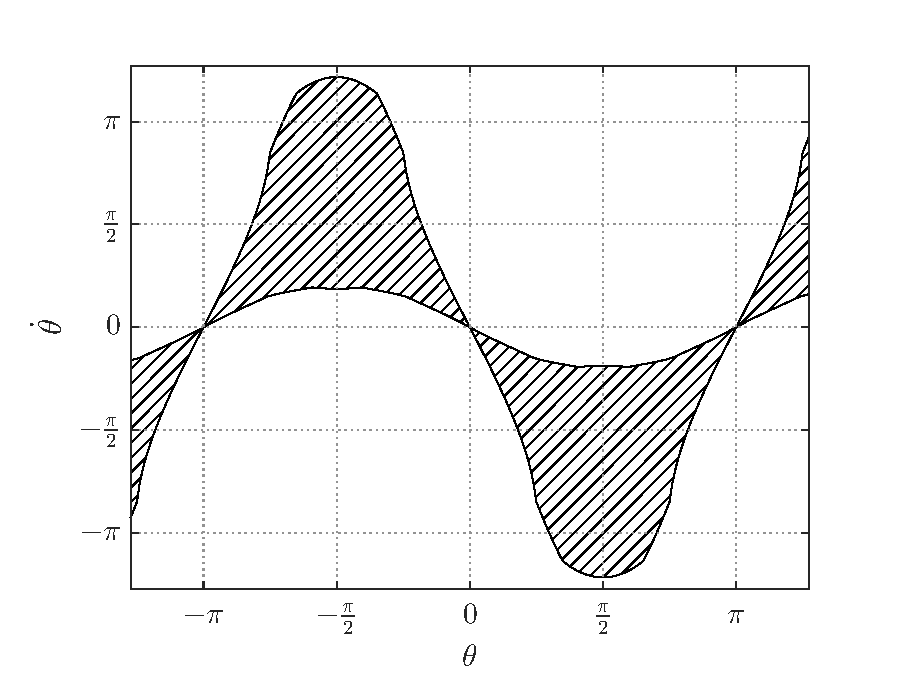
\includegraphics[width=1\linewidth]{fig/omega_bounds}
    \caption{Example angular velocity bounds for the 2D tetrapod from
      Figure \ref{fig:moment-envelope}. The tetrapod is oriented such
      that the stable pulling configuration corresponds to
      $\theta=0$.}
  \label{fig:omega-bounds}
\end{figure}

The angular velocity bounds derived in section
\ref{sec:exact-angular-velocity-bounds} can be integrated into bounds
on the position of the pulled body.  Let $\theta$ be the true
orientation of the pulled body in the world frame. Let the function
$\omega$ map from the pulling angle to the true angular
velocity. Likewise, let $u$ and $l$ be upper and lower bounds on the
true orientation, and let the functions $\alpha$ and $\beta$ map from
the pulling angle to the upper and lower angular velocity bounds. An
example plot of $u$ and $l$ is illustrated in Figure
\ref{fig:omega-bounds}.

We assume that the pulling trajectory
$\gamma:\mathbb{R}\rightarrow\mathbb{R}^2$ can be approximated by a
finite number of straight line segments of equal length. Given such a
$\gamma$, the pulling angle
$\phi(t) = \tan^{-1}(\gamma_y(t),\gamma_x(t))$ is a piece-wise
constant (step) function. As the planar rigid body is pulled along
$\gamma$, the variables $\theta$, $u$, $\ell$ change according to the
dynamical system
\begin{align}
  \dot{\theta} &= \omega(\theta - \phi(t))\\
  \dot{u} &=  \alpha(u - \phi(t)) \label{eq:u-ode}\\ 
  \dot{\ell} &=  \beta(\ell - \phi(t)). 
\end{align}
Without loss of generality, we assume that the body is pulled at a
constant unit velocity.

\begin{proposition}
  For pulling of a rigid body with known initial pose, the orientation
  of the body is bounded above and below by $u$ and $\ell$.
\end{proposition}

\begin{proof}
  Suppose the proposition is false and $\theta$ crosses the bound $u$
  at time $t_0$, i.e. $u(t_0)=\theta(t_0)$ and $\theta(t) > u(t)$
  immediately afterwards. Let the line segment of $\gamma$ at $t_0$ be
  indexed by $i$ and have length $\varepsilon$. Then $\phi(t)$ is
  constant for $t$ in the range $[t_0,(i+1)\varepsilon)$. Pick $t_1$
  from said range such that $\theta(t_1) > u(t_1)$. Because $\phi$ is
  constant in $[t_0,t_1]$, we can apply separation of variables to
  solve differential equation (\ref{eq:u-ode}) and get
  \begin{equation}
    \int_{u(t_0)}^{u(t_1)}\frac{1}{\alpha(x - \phi(t_0))}dx = \int_{t_0}^{t_1}dt.
  \end{equation}
  This result shows that we can integrate the inverse of an angular
  velocity function to compute the amount of time required to reach a
  particular orientation. However, we can also apply separation of
  variables to the function $\omega$. Observe that because $\alpha$ is
  an upper bound
  \begin{equation} 
    \alpha(x - \phi(t_0)) \geq \omega(x - \phi(t_0)),
  \end{equation}
  the resulting integral of $\omega$ satisfies
  \begin{equation}
    \int_{u(t_0)}^{u(t_1)}\frac{1}{\alpha(x - \phi(t_0))}dx \leq \int_{u(t_0)}^{u(t_1)}\frac{1}{\omega(x - \phi(t_0))}dx.
  \end{equation}
  This indicates that $\theta(t_1) \leq u(t_1)$, a
  contradiction. Therefore, the upper bound holds and the lower bound
  follows from an identical argument.
\end{proof}

% \begin{proposition}
%   The angular velocity bounds on the motion of the pulled body are
%   continuous with respect to the orientation.
% \end{proposition}

% \begin{proof}
%   \TODO{
%     Sketch of proof idea:
%     \begin{enumerate}
%     \item A sequence of continuous functions which converges uniformly
%       to the lower bound $\alpha$ $\Rightarrow$ $\alpha$ is
%       continuous.
%     \item To construct such a sequence:
%     \item For all $N\in\mathcal{N}$, take $N$ evenly spaced points in
%       $[-\pi,\pi]$.
%     \item Can construct continuous function that approximates $\alpha$
%       by picking a minimum generating pressure distribution for each
%       $\theta_i$ and interpolating continuously between each
%       $\alpha(\theta_i)$.
%     \item If we can show the interpolating function has bounded
%       subgradient, then we can show it converges uniformly to
%       $\alpha$.
%     \item Intuitively we should be able to pick pressures $p_i$ and
%       $p_{i+1}$ for orientations $\theta_i$ and $\theta_{i+1}$ such
%       that they are ``close'' together. Then we need to show that
%       $p_i$ and $p_{i+1}$ being close implies that their minimizing
%       angular velocities are close in a global sense.
%     \item ?????
%     \end{enumerate}
%   }
% \end{proof}


\subsection{Differential Dynamic Programming}

\begin{proposition}
  $\mathcal{u}\mathcal{L} \times \mathcal{U}$ $\Omega \Phi$ $u \ell U L \alpha \beta A B $

\begin{align*}
  \dot x &= x \\
  \dot y &= y \\
  \dot\ell &= \alpha() \\
  \dot u &= \beta() 
\end{align*}

  $\dot{\theta}_u = u()$

  $\dot{\theta}_\ell = \ell()$
\end{proposition}

\section{Implementation}

\subsection{Hardware}

\subsection{MATLAB}

\section{Experiments}

\subsection{Exact Bounds vs Peshkin's Bound}
\begin{enumerate}
\item MIT Dataset objects' aspect ratios are lacking.
\item Alexander and Maddock omitted because...
\item Turn faster for smaller objects?
\end{enumerate}

\section{Discussion}

\section{Conclusion}

\bibliographystyle{plainnat}
\bibliography{references}

\end{document}
